\section{Umgang mit JIRA-Tickets}
In diesem Artikel wird beschrieben, welche Funktionen die jeweiligen Tickets im Jira erfüllen und wann diese eingesetzt werden. Man unterscheidet zwischen Epics, User-Stories, Tasks, Sub-Tasks und Bugs.
\begin{figure}[!ht]
	\centering
	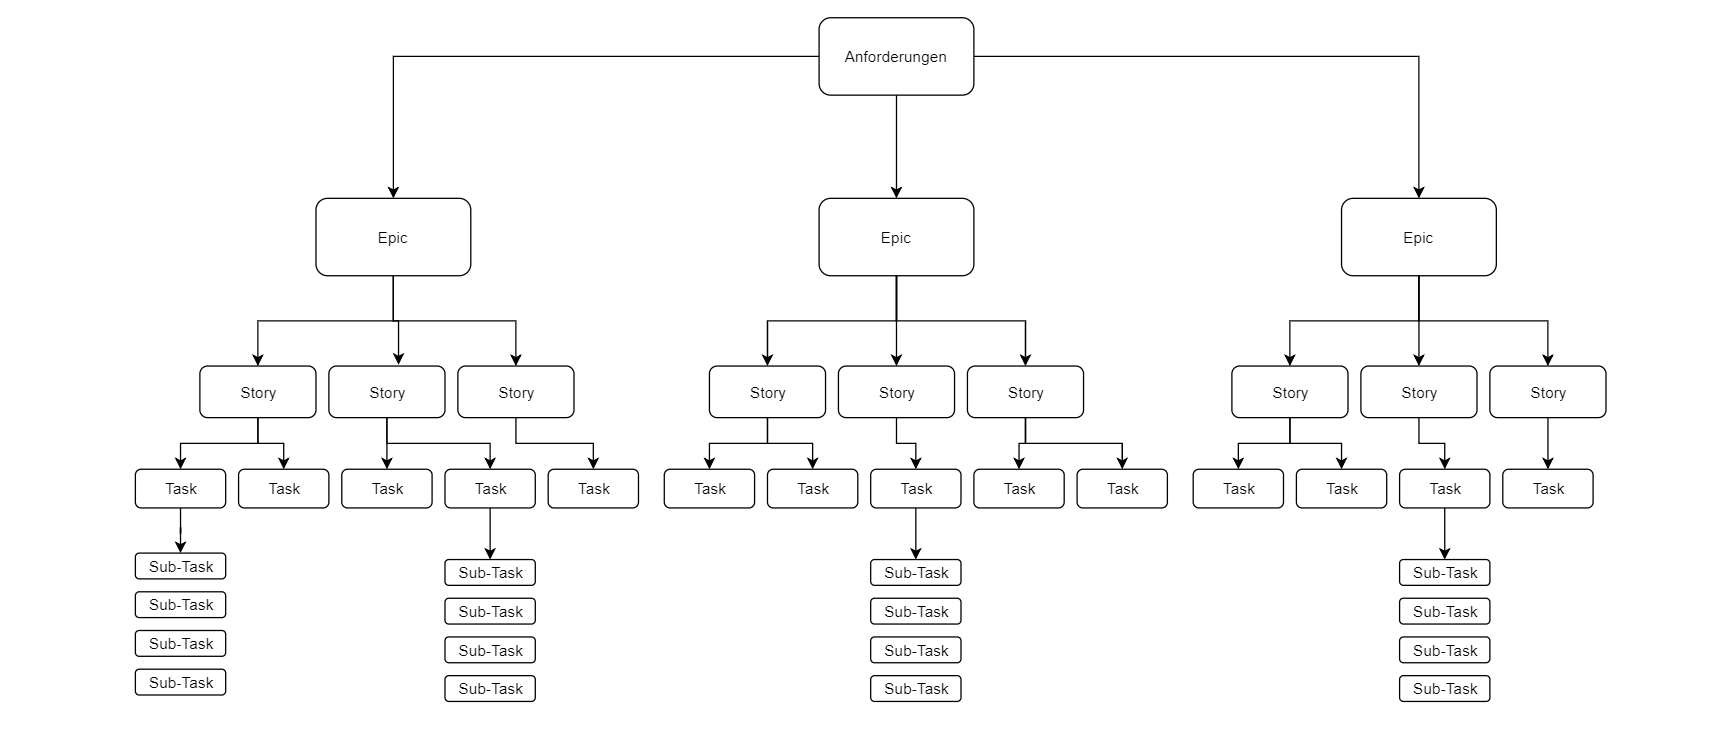
\includegraphics[width=\textwidth]{./ressourcen/jira-hierarchie.png}
	\caption{Hierarchie der "`issue types"' in JIRA}
\end{figure}

\subsection{Epic}
Das Epic das Thema der Umsetzung. Diese wird beispielsweise angelegt, wenn eine neue Funktion in eine Software eingebaut werden soll.\cite{atlassian:jira-support} \\
Ein Epic bildet üblicherweise das Thema einer neuen Umsetzung. Dabei werden die konkreten Anforderungen nicht in einem Epic beschrieben, sondern als zusätzliche Story- oder Task-Tickets formuliert und dann mit dem Epic verlinkt. Das Epic dient also nur der Zusammenfassung aller zugehörigen Anforderungenbei einer größeren Umsetzung von Features oder Ähnlichem.\cite{atlassian:jira-support}

\subsection{User Story}
In einer User-Story werden einzelne Anforderungen aus Sicht des Kunden beschrieben. Die Stories können dann einem Bearbeiter zugewiesen werden, welcher für die Umsetzung der Anforderungen in dem Story-Ticket verantwortlich ist. Zudem können einem Story-Ticket eine "`Defintion of Done"' (DoD), "`Definition of Ready"'  oder andere Kriterien hinzugefügt werden. Anhand der DoD kann der Entwickler zum Beispiel während oder nach der Bearbeitung des Tickets überprüfen, ob er alle ihm zugeordneten Aufgaben erfüllt hat, welche im Zusammenhang mit der Story stehen. Dazu kann zum Beispiel das Erstellen eines Tests gehören oder die korrekte Dokumentation. \cite{scrum-guide}

\subsection{Task}
Bei einer Task werden die User-Stories in weitere Aufgaben zerlegt. Wenn eine Aufgabe eine vereinbarte Zeitspanne überschreitet, kann sie in zusätzliche Aufgaben (Sub-Tasks) aufgeteilt werden. Eine User Story ist dann erledigt, wenn alle beinhaltete Aufgaben erledigt sind. \cite{atlassian:jira-support}
